%%%%%%%%%%%%%%%%%%%%%%%%%%%%%%%%%%%%%%%%%%%%%%%%%%%%%%%%%%%%%%%%%%
\section{Evaluation}									%%%%%%%%%%
\label{evaluation}										%%%%%%%%%%
%%%%%%%%%%%%%%%%%%%%%%%%%%%%%%%%%%%%%%%%%%%%%%%%%%%%%%%%%%%%%%%%%%
% Experimental setup
All experiments are run on a 10 node cluster with 18 object storage daemons (OSDs), 1 monitor node (MON), and up to 5 MDS nodes. Each node is running Ubuntu 12.04.4 (kernel version 3.2.0-63) and they have 2 dual core 2GHz processors and 8GB of RAM. There are 3 OSDs per physical server and each OSD has its own disk formatted with XFS for data and an SSD partition for its journal. We use Ceph version 0.91-365-g2da2311. Before each experiment, the cluster is torn down and re-initialized and the kernel caches on all OSDs, MDS nodes, and clients are dropped. 

Performance numbers are specific to CephFS but our contribution is the balancing API/framework that allows users to study different strategies {\it on the same storage system}.  Furthermore, we are not arguing that Mantle is more scalable or better performing than GIGA+, rather, we want to highlight its strategy in comparison to other strategies using Mantle. While it is natural to compare raw performance numbers, we feel (and not just because GIGA+ outperforms Mantle) that we are attacking an orthogonal issue by providing a system for which we can test the strategies of the systems, rather than the systems themselves. 

% Workload discussion
\textbf{Workloads}: we use a small number of workloads to show a comprehensive view of how load is split across MDS nodes. We use file-create workloads because they stress the system, are the focus of other state-of-the-art metadata systems, and they are a common HPC problem (checkpoint/restart). We use compiling code as the other workload because it has different metadata request types/frequencies and because users plan to use CephFS as a shared file system~\cite{website:ceph-cephfs-product-release}. Initial experiments with 1 client compiling with 1 MDS are, admittedly, not interesting, but we use it as a baseline for comparing against setups with more clients. 

% Metrics discussion
\textbf{Metrics}: Mantle pulls out metrics that could be important so that the administrator can freely explore them. The metrics we use are instantaneous CPU utilization and metadata writes, but future balancers will use metrics that better indicate load and that have less variability. In this paper, the high variance in the measurements influences the results of our experiments.

% Balancer design discussion
\textbf{Balancing Heuristics}: we use Mantle to explore techniques from related work: ``Greedy Spill" is from GIGA+, ``Fill \& Spill" is a variation of LARD~\cite{pai:asplos1998}, and the ``Adaptable Balancer" is the original CephFS policy. These heuristics are just starting points and we are not ready to make grandiose statements about which is best. 

%%%%%%%%%%
\subsection{Greedy Spill Balancer}
\label{greedy-spill-balancer}
%%%%%%%%%%
% /user/msevilla/results/sc/spill-evenly
\begin{figure}[tb]
	\centering	
	%\includegraphics[width=0.4\textwidth]{./figures/eval_spill-evenly.pdf}
   	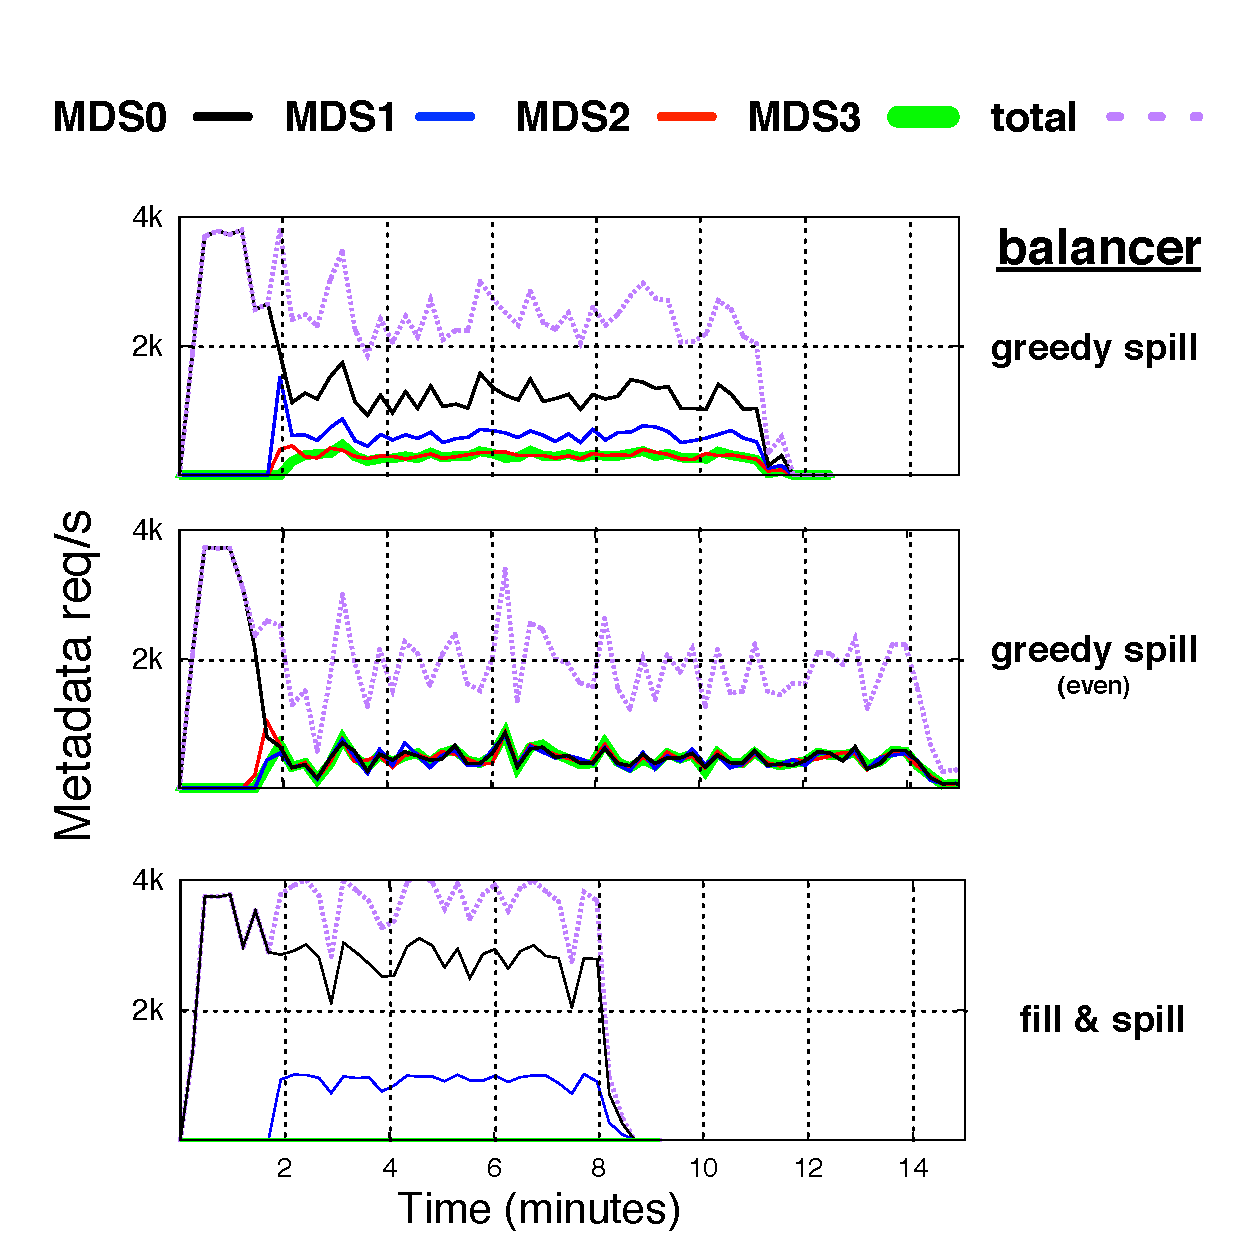
\includegraphics[width=0.4\textwidth]{./chapters/mantle/figures/spill-evenly.pdf}
	\caption{With clients creating files in the same directory, spilling load unevenly with Fill \& Spill has the highest throughput (curves are not stacked), which can have up to 9\% speedup over 1 MDS. Greedy Spill sheds half its metadata immediately while Fill \& Spill sheds part of its metadata when overloaded.\label{figure:eval_spill-evenly}}
\end{figure}
\begin{figure}[tb]
	\centering	
	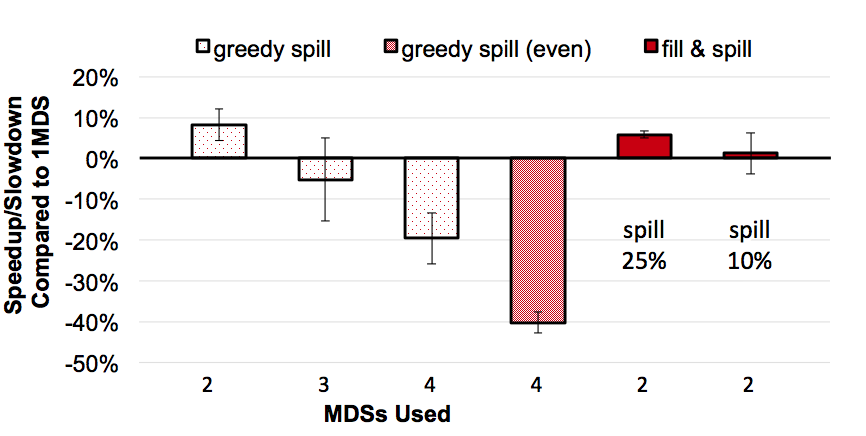
\includegraphics[width=0.4\textwidth]{./chapters/mantle/figures/eval_spill-evenly_bar}
	\caption{The per-client speedup or slowdown shows whether distributing metadata is worthwhile.  Spilling load to 3 or 4 MDS nodes degrades performance but spilling to 2 MDS nodes improves performance.\label{figure:eval_spill-evenly_bar}}
\end{figure}

% overview
This balancer, shown in Listing~\ref{listing:greedy-spill}, aggressively sheds load to all MDS nodes and works well for many clients creating files in the same directory. This balancing strategy mimics the uniform hashing strategy of GIGA+~\cite{patil:fast2011-giga+, ren:sc2014-indexfs}. In these experiments, we use 4 clients each creating 100,000 files in the same directory. When the directory reaches 50,000 directory entries, it is fragmented (the first iteration fragments into \(2^{3}\) = 8 dirfrags) and the balancer migrates half of its dirfrags to an ``underutilized" neighbor. 

\begin{listing}
	\begin{minted}[frame=lines]{lua}
-- Metadata load
metaload = IWR
-- Metadata server load
mdsload = MDSs[i]["all"]
-- When policy
if MDSs[whoami]["load"]>.01 and 
   MDSs[whoami+1]["load"]<.01 then
-- Where policy
targets[whoami+1]=allmetaload/2
-- Howmuch policy
{"half"}
	\end{minted}
    \caption{Greedy Spill Balancer using the Mantle environment (listed in Table~\ref{table:metrics}). Note that all subsequent balancers use the same metadata and MDS loads.\label{listing:greedy-spill}}
\end{listing}

% describe injectable code
The metadata load for the subtrees/dirfrags in the namespace is calculated using just the number of inode writes; we focus on create-intensive workloads, so inode reads are not considered. The MDS load for each MDS is based solely on the metadata load. The balancer migrates load (``when") if two conditions are satisfied: the current MDS has load to migrate and the neighbor MDS does not have any load. If the balancer decides to migrate, it sheds half of the load to its neighbor (``where"). Finally, to ensure that exactly half of the load is sent at each iteration, we employ a custom fragment selector that sends half the dirfrags (``howmuch"). 

% describe results 
The first graph in Figure~\ref{figure:eval_spill-evenly} shows the instantaneous throughput ({\it y} axis) of this balancer over time ({\it x} axis). The MDS nodes spill half their load as soon as they can - this splits load evenly for 2 MDS nodes, but with 4 MDS nodes the load splits unevenly because each MDS spills less load than its predecessor MDS. To get the even balancing shown in the second graph of Figure~\ref{figure:eval_spill-evenly}, the balancer is modified according to Listing~\ref{listing:greedy-spill-evenly} to partition the cluster when selecting the target MDS.
\begin{listing}
	\begin{minted}[frame=lines]{lua}
-- When policy
t=((#MDSs-whoami+1)/2)+whoami
if t>#MDSs then t=whoami end
while t~=whoami and MDSs[t]<.01 do t=t-1 end
if MDSs[whoami]["load"]>.01 and        
   MDSs[t]["load"]<.01 then
-- Where policy
targets[t]=MDSs[whoami]["load"]/2
	\end{minted}
    \caption{Greedy Spill Evenly Balancer.\label{listing:greedy-spill-evenly}}
\end{listing}

% injectable code
This change makes the balancer search for an underloaded MDS in the cluster. It splits the cluster in half and iterates over a subset of the MDS nodes in its search for an underutilized MDS. If it reaches itself or an undefined MDS, then it has nowhere to migrate its load and it does not do any migrations. The ``where" decision uses the target, \texttt{t}, discovered in the ``when" search. With this modification, load is split evenly across all 4 MDS nodes.

% the overall results
The balancer with the most speedup is the 2 MDS configuration, as shown in Figure~\ref{figure:eval_spill-evenly_bar}. This agrees with the assessment of the capacity of a single MDS in Section~\S\ref{setting-policies-for-migration-decisions}; at 4 clients, a single MDS is only slightly overloaded, so splitting load to two MDS nodes only improves the performance by 10\%. Spilling unevenly to 3 and 4 MDS nodes degrades performance by 5\% and 20\% because the cost of synchronizing across multiple MDS nodes penalizes the balancer enough to make migration inefficient. Spilling evenly with 4 MDSs degrades performance up to 40\%  but has the lowest standard deviation because the MDS nodes are underutilized.

% explain the reasons for the poor performance
The difference in performance is dependent on the number of flushes to client sessions. Client sessions ensure coherency and consistency in the file system ({\it e.g.,} permissions, capabilities, etc.) and are flushed when slave MDS nodes rename or migrate directories\footnote{The cause of the latency could be from a scatter-gather process used to exchange statistics with the authoritative MDS. This requires each MDS to halt updates on that directory, send the statistics to the authoritative MDS, and then wait for a response with updates.}: 157 sessions for 1 MDS, 323 session for 2 MDS nodes, 458 sessions for 3 MDS nodes, 788 sessions for 4 MDS nodes spilled unevenly, and 936 sessions for 4 MDS nodes with even metadata distribution. There are more sessions when metadata is distributed because each client contacts MDS nodes round robin for each create. This design decision stems from CephFS's desire to be a general purpose file system, with coherency and consistency for shared resources.\\

\noindent\textbf{Performance}: migration can have such large overhead that the parallelism benefits of distribution are not worthwhile.\\
\noindent\textbf{Stability}: distribution lowers standard deviations because MDS nodes are not as overloaded.

%%%%%%%%%%%%%%%%%%%%%%%%%%%%%%%%%%%%%%%%%%%%%%%%%%%%%%%%%%%%%%%%%%
\subsection{Fill and Spill Balancer}					%%%%%%%%%%
\label{fill-and-spill-balancer}							%%%%%%%%%%
%%%%%%%%%%%%%%%%%%%%%%%%%%%%%%%%%%%%%%%%%%%%%%%%%%%%%%%%%%%%%%%%%%
% overview
This balancer, shown in Listing~\ref{listing:fill-and-spill}, encourages MDS nodes to offload inodes {\it only} when overloaded.  Ideally, the first MDS handles as many clients as possible before shedding load, increasing locality and reducing the number of forwarded requests. Figuring out when an MDS is overloaded is a crucial policy for this balancer. In our implementation, we use the MDS's instantaneous CPU utilization as our load metric, although we envision a more sophisticated metric built from a statistical model for future work. To figure out a good threshold, we look at the CPU utilization from the scaling experiment in Section~\S\ref{setting-policies-for-migration-decisions}. We use the CPU utilization when the MDS has 3 clients, about 48\%, since 5, 6, and 7 clients appear to overload the MDS.  

\begin{listing}
	\begin{minted}[frame=lines]{lua}
-- When policy
wait=RDState(); go = 0;
if MDSs[whoami]["cpu"]>48 then
  if wait>0 then WRState(wait-1)
  else WRState(2); go=1; end
else WRState(2) end
if go==1 then
-- Where policy
targets[whoami+1] = MDSs[whoami]["load"]/4
	\end{minted}
    \caption{Fill and Spill Balancer.\label{listing:fill-and-spill}}
\end{listing}
% injectable code
The injectable code for both the metadata load and MDS load is based solely on the inode reads and writes. The ``when" code forces the balancer to spill when the CPU load is higher than 48\% for more than 3 straight iterations. We added the ``3 straight iterations'' condition to make the balancer more conservative after it had already sent load; in early runs the balancer would send load, then would receive the remote MDS's heartbeat (which is a little stale) and think that the remote MDS is {\it still underloaded}, prompting the balancer to send more load. Finally, the ``where" code tries to spill small load units, just to see if that alleviates load enough to get the CPU utilization back down to 48\%. 

% results
This balancer has a speedup of 6\% over 1 MDS, as shown in Figure~\ref{figure:eval_spill-evenly_bar}, and only uses a subset of the MDS nodes. With 4 available MDS nodes, the balancer only uses 2 of them to complete the job, which minimizes the migrations and the number of sessions. The experiments also show how the amount of spilled load affects performance. Spilling 10\% has a longer runtime, indicating that MDS0 is slightly overloaded when running at 48\% utilization and would be better served if the balancer had shed a little more load. In our experiments, spilling 25\% of the load has the best performance.\\

\noindent\textbf{Performance}: knowing the capacity of an MDS increases performance using only a subset of the MDS nodes.\\
\noindent\textbf{Stability}: the standard deviation of the runtime increases if the balancer compensates for poor migration decisions.

%%%%%%%%%%%%%%%%%%%%%%%%%%%%%%%%%%%%%%%%%%%%%%%%%%%%%%%%%%%%%%%%%%
\subsection{Adaptable Balancer}						%%%%%%%%%%
\label{adaptable-balancer}								%%%%%%%%%%
%%%%%%%%%%%%%%%%%%%%%%%%%%%%%%%%%%%%%%%%%%%%%%%%%%%%%%%%%%%%%%%%%%
\begin{figure}[t]
	\centering	
	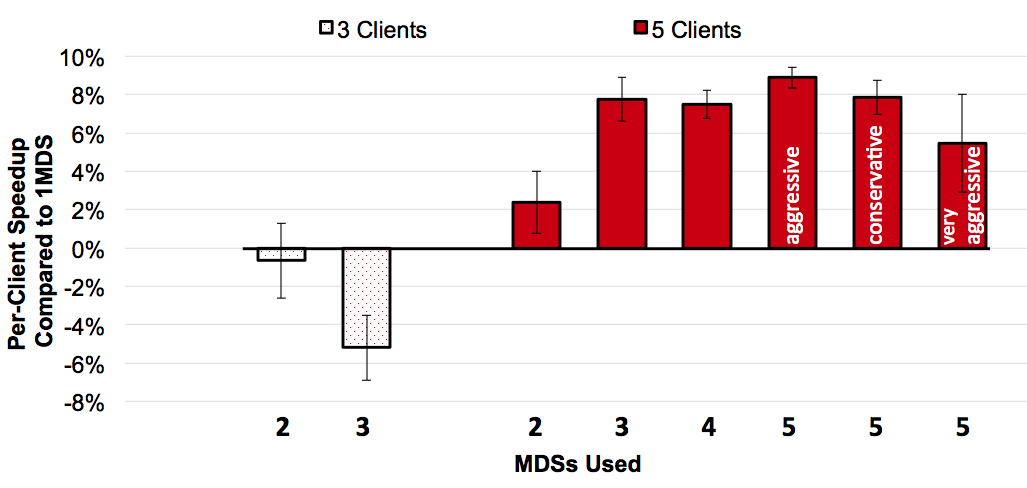
\includegraphics[width=0.5\textwidth]{./chapters/mantle/figures/eval_spill-evenly_compile_bar}\caption{For the compile workload, 3 clients do not overload the MDS nodes so distribution is only a penalty. The speedup for distributing metadata with 5 clients suggests that an MDS with 3 clients is slightly overloaded.  \label{figure:eval_spill-evenly_compile_bar}}
\end{figure}
\begin{figure}[tb]
	\centering	
	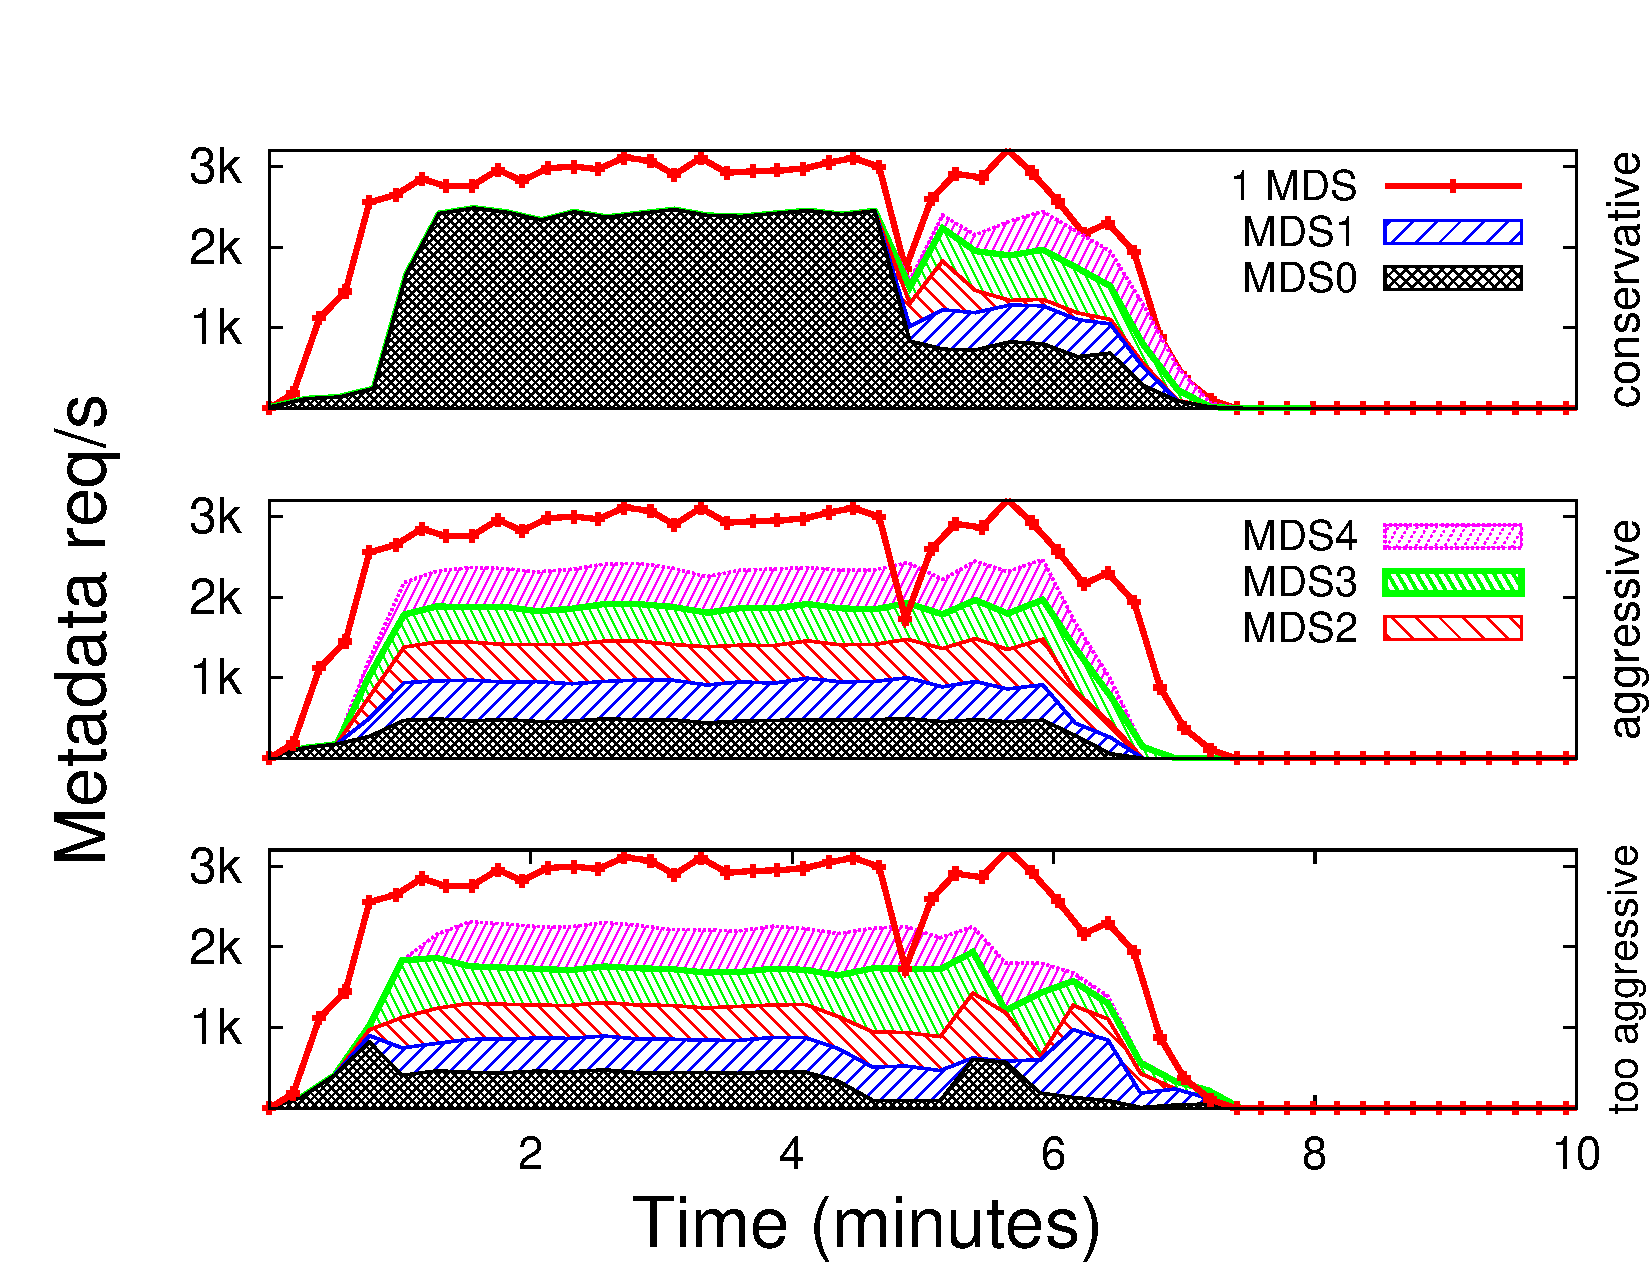
\includegraphics[width=0.45\textwidth]{./chapters/mantle/figures/eval_spill-evenly_compile}\caption{With 5 clients compiling code in separate directories, distributing metadata load early helps the cluster handle a flash crowd at the end of the job. Throughput (stacked curves) drops when using 1 MDS (red curve) because the clients shift to linking, which overloads 1 MDS with \texttt{readdir}s.\label{figure:eval_spill-evenly_compile}}
\end{figure}

This balancer, shown in Listing~\ref{listing:adaptable}, migrates load frequently to try and alleviate hotspots. It works well for dynamic workloads, like compiling code, because it can adapt to the spatial and temporal locality of the requests. The adaptable balancer uses a simplified version of the adaptable load sharing technique of the original balancer.

\begin{listing}
	\begin{minted}[frame=lines]{lua}
-- Metadata load
metaload = IWR + IRD
-- When policy
max=0
for i=1,#MDSs do
  max = max(MDSs[i]["load"], max)
end
myLoad = MDSs[whoami]["load"]
if myLoad>total/2 and myLoad>=max then
-- Balancer where policy
targetLoad=total/#MDSs
for i=1,#MDSs do
  if MDSs[i]["load"]<targetLoad then
    targets[i]=targetLoad-MDSs[i]["load"]
  end
end
-- Howmuch policy
{"half","small","big","big_small"}
	\end{minted}
    \caption{Adaptable Balancer.\label{listing:adaptable}}
\end{listing}

% explain the code
Again, the metadata and MDS loads are set to be the inode writes (not shown). The ``when'' condition only lets the balancer migrate load if the current MDS has more than half the load in the cluster and if it has the most load. This restricts the cluster to only one exporter at a time and only lets that exporter migrate if it has the majority of the load. This makes the migrations more conservative, as the balancer will only react if there is a single MDS that is severely overloaded. The ``where'' code scales the amount of load the current MDS sends according to how much load the remote MDS has. Finally, the balancer tries to be as accurate as possible for all its decisions, so it uses a wide range of dirfrag selectors.

% the results
Figure~\ref{figure:eval_spill-evenly_compile_bar} shows how Mantle can spread load across MDS nodes in different ways. That figure shows the overall performance for 5 clients compiling the Linux source code in separate directories. The balancer immediately moves the large subtrees, in this case the root directory of each client, and then stops migrating because no single MDS has the majority of the load. We conclude that 3 clients do not saturate the system enough to make distribution worthwhile and 5 clients with 3 MDS nodes is just as efficient as 4 or 5 MDS nodes. 

% The performance profile
The performance profile for the 5 MDS setups in Figure~\ref{figure:eval_spill-evenly_compile} shows how the aggressiveness of the balancer affects performance. The bold red curve is the metadata throughput for the compile job with 1 MDS and the stacked throughput curves correspond to the same job with 5 MDS nodes. The top balancer sets a minimum offload number, so it behaves conservatively by keeping all metadata on one MDS until a metadata load spike at 5 minutes forces distribution. The middle balancer is aggressive and distributes metadata load immediately. The flash crowd that triggers the migration in the top graph does not affect the throughput of the aggressive balancer, suggesting that the flash crowd requests metadata that the single MDS setup cannot satisfy fast enough; metadata is subsequently distributed but the flash crowd is already gone. The bottom balancer is far too aggressive and it  tries to achieve perfect balance by constantly moving subtrees/dirfrags. As a result, performance is worse (60\(\times\) as many forwards as the middle balancer), and the standard deviation for the runtime is much higher.\\

\noindent\textbf{Performance}: adapting the system to the workload can improve performance dramatically, but aggressively searching for the perfect balance hurts performance.\\
\noindent\textbf{Stability}: a fragmented namespace destroys locality and influences the standard deviation dramatically.\\
\noindent\textbf{Overhead}: the gap between the 1 MDS curve and the MDS0 curve in the top graph in Figure~\ref{figure:eval_spill-evenly_compile} is the overhead of the balancing logic, which includes the migration decisions, sending heartbeats, and fragmenting directories. The effect is significant, costing almost 500 requests per second, but should be dulled with more MDS nodes if they make decisions independently.

%%%%%%%%%%%%%%%%%%%%%%%%%%%%%%%%%%%%%%%%%%%%%%%%%%%%%%%%%%%%%%%%%%
\subsection{Discussion and Future Work}
\label{discussion-future-work}
%%%%%%%%%%%%%%%%%%%%%%%%%%%%%%%%%%%%%%%%%%%%%%%%%%%%%%%%%%%%%%%%%%
In this paper we only show how certain policies can improve or degrade performance and instead focus on how the API is flexible enough to express many strategies.  While we do not come up with a solution that is better than state-of-the-art systems optimized for file creates ({\it e.g.}, GIGA+), we do present a framework that allows users to study the emergent behavior of different strategies, both in research and in the classroom. In the immediate future, we hope to quantify the effect that policies have on performance by running a suite of workloads over different balancers. Other future endeavors will focus on:

\textbf{Analyzing Scalability}: our MDS cluster is small, but today's production systems use metadata services with a small number of nodes (often less than 5)~\cite{website:ceph-cephfs-product-release}. Our balancers are robust until 20 nodes, at which point there is increased variability in client performance for reasons that we are still investigating. We expect to encounter problems with CephFS's architecture ({\it e.g.}, n-way communication and memory pressure with many files), but we are optimistic that we can try other techniques using Mantle, like GIGA+'s autonomous load splitting, because Mantle MDS nodes independently make decisions. 

%Mantle has already exposed 2 performance deficiencies in CephFS, so it can also help improve metadata protocols and system architectures.	

\textbf{Adding Complex Balancers}: the biggest reason for designing Mantle is to be able to test more complex balancers. Mantle's ability to save state should accommodate balancers that use request cost and statistical modeling, control feedback loops, and machine learning.

\textbf{Analyzing Security and Safety}: in the current prototype, there is little safety - the administrator can inject bad policies ({\it e.g.}, \texttt{while 1}) that brings the whole system down. We wrote a simulator that checks the logic before injecting policies in the running cluster, but this still needs to be integrated into the prototype.


